\chapter{Função do segundo grau}

\section{Introdução}

No capítulo sobre função de 1º grau foram estudados modelos em que as grandezas eram simplesmente proporcionais entre si. Isto significa que, para o mesmo incremento \textit{($ \Delta $ x) }em qualquer \textit{x}, o incremento \textit{($ \Delta $ y) }em \textit{y}, será sempre o mesmo. Os gráficos dessas funções são retas. Porém, muitas grandezas se relacionam proporcionalmente ao quadrado de outras: é o caso da área de um quadrado em relação ao lado; a área de um círculo em relação ao raio; o deslocamento de uma pedra em queda livre em relação ao tempo e muitas outras. Estas funções são chamadas de quadráticas e serão estudadas neste capítulo. 

\section{Definição de função do 2º grau }

As funções polinomiais tem a forma 

 \( f \left( x \right) =a_{0}+a_{1}x+a_{2}x^{2}+a_{3}x^{3}+a_{4}x^{4}+ \ldots +a_{n}x^{n} \) \tab (2.1)

onde \textit{a\textsubscript{i}} são números reais, para \textit{i = 0,1,2,3,4, ...n}.

O grau de uma função polinomial é dado pelo maior grau do polinômio. Assim,

\begin{enumerate}
	\item  \( f \left( x \right) = a_{0}+a_{1}x \)    é uma função do 1º grau, para    \textit{a\textsubscript{1} $ \neq $  0  .}

	\item  \( f \left( x \right) =a_{0}+a_{1}x+a_{2}x^{2} \)    é uma função do 2º grau, para    \textit{a\textsubscript{2} $ \neq $  0 . }

	\item  \( f \left( x \right) =a_{0}+a_{1}x+a_{2}x^{2}+a_{3}x^{3} \)    é uma função do 3º grau, para    \textit{a\textsubscript{3} $ \neq $  0  }

	\item  \( f \left( x \right) =a_{0}+a_{1}x+a_{2}x^{2}+a_{3}x^{3}+ \ldots +a_{n}x^{n} \)       é uma função do grau \textit{n}, para    \textit{a\textsubscript{n} $ \neq $  0  .}
\end{enumerate}

Particularmente, as funções de 2º grau (também chamadas de \textit{funções quadráticas}) tem a forma:  

 \( f \left( x \right) =a_{0}+a_{1}x+a_{2}x^{2} \) , para    \textit{a\textsubscript{2} $ \neq $  0  }. (2.2)

Para simplificar a notação (evitar sub-índices), vamos substituir \textit{a\textsubscript{0} = C,   a\textsubscript{1} = B}    e    \textit{a\textsubscript{2} = A}   na Eq. (2.2) e obter :

 \( f \left( x \right) =Ax^{2}+Bx+C_{~ } \) , para \textit{A $ \neq $  0  }.\tab (2.3)

\begin{texemplo}
a) Na função  \( f \left( x \right) =x^{2}+2x-3_{~ } \)  \textit{, A=1; B=2 }e\textit{ C=-3}.

b) Na função  \( g \left( x \right) =3x^{2}-1/3_{~ } \)  \textit{, A=3; B=0 }e\textit{ C=-1/3}.

c) Na função  \( h \left( x \right) =-x^{2}+5x_{~ } \)  \textit{, A=-1; B=5 }e\textit{ C=0}.

d) Na função  \( p \left( x \right) =-3x^{2}_{~ } \)  \textit{, A=-3; B=0 }e\textit{ C=0 }\qedsymbol{}
\end{texemplo}

\section{Gráfico de uma função de 2º grau}

O modo mais elementar de fazer o gráfico de uma função do 2º grau conhecida é localizando vários pontos da função no plano cartesiano. Esse modo é simples e fácil, porém demorado e mecânico. Vejamos um exemplo:

\begin{texemplo}
Faça o gráfico da função  \textit{f(x) = x\textsuperscript{2} - 4}x.

\textbf{Solução}: Podemos fazer uma tabela atribuindo valores para \textit{x} e calculando os correspondentes valores de \textit{f(x)} com a função dada.

\begin{figure}[H]
	\begin{Center}
		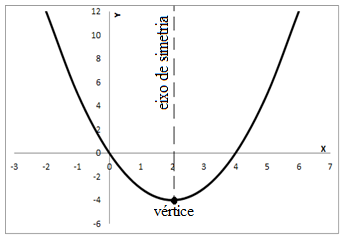
\includegraphics[width=3.56in,height=2.46in]{capitulos/funcao_do_segundo_grau/media/image2.png}
	\end{Center}
\end{figure}

Observemos que o gráfico de \textit{f(x)} é uma \textit{curva}. As curvas resultantes de funções de 2º grau são chamadas \textit{PARÁBOLAS}. 

Observemos também que as parábolas têm um \textbf{\textit{eixo de simetria}} que divide a curva em duas partes iguais, o qual passa pelo \textbf{\textit{vértice}} (ponto extremo da curva). 

Como sugestão de atividade, incentivamos o leitor a obter o gráfico do presente exemplo em uma planilha eletrônica \qedsymbol{}
\end{texemplo}

\subsection{Concavidade da parábola}

As parábolas com a forma da Eq. (2.3) têm \textbf{\textit{concavidade para cima ou para baixo}}.

\begin{caixa}
Se \textit{A > 0}  então a concavidade é para cima

Se \textit{A < 0}  então a concavidade é para baixo.
\end{caixa}

\begin{texemplo}
Faça um esboço do gráfico das funções \textit{f(x) = x\textsuperscript{2} } e  \textit{g(x) = - x\textsuperscript{2} } . 

\textbf{Solução}: Atribuindo valores para \textit{x} e calculando os correspondentes valores de \textit{f(x)} e \textit{g(x)  }obtemos os gráficos das figuras abaixo.

\begin{figure}[H]
    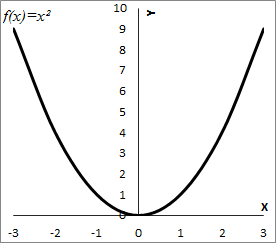
\includegraphics[width=0.45\textwidth]{capitulos/funcao_do_segundo_grau/media/image3.png}

    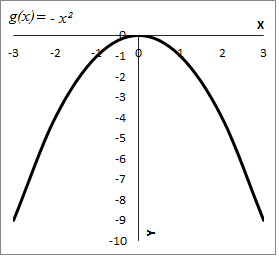
\includegraphics[width=0.45\textwidth]{capitulos/funcao_do_segundo_grau/media/image4.png}
\end{figure}

Observemos que para  \textit{A > 0}   a concavidade é para cima e para \textit{A < 0}  a concavidade é para baixo\qedsymbol{}
\end{texemplo}

\subsection{Intersectação com o eixo Y}

Os pontos onde qualquer função intersecta o eixo Y tem abcissa igual a zero (\textit{x=0}). Fazendo \textit{x=0}  na Eq. (2.3) temos:

 \( y=A0^{2}+B0+C_{~ } \)

\textit{y = C.} \tab (3.1)

Portanto, a parábola vai intersectar o eixo \textit{Y} em (\textit{0,C}).

\subsection{Raízes das funções de 2º grau (intersectação com o eixo X)}

Lembremos que a raiz de uma função é o valor da abcissa (\textit{x\textsubscript{r}}) do ponto em que a função intersecta o eixo \textit{X}, portanto, nesse ponto temos \textit{y = 0}. 

Fazendo \textit{y = f(x) = 0}  na Eq. (2.3) temos uma equação de 2º grau:

   \( 0=Ax^{2}+Bx+C_{~ } \) \tab (3.2)

A solução da Eq. (3.2) foi demonstrada no capítulo sobre equações, cuja conclusão  é a fórmula de Baskhara:

 \( x_{1,2}=\frac{-B \pm \sqrt[]{B^{2}-4AC}}{2A} \) \tab (3.3)

\begin{texemplo}
Calcule as raízes e faça um esboço do gráfico da função \textit{f(x) = x\textsuperscript{2} -x -6} . 

\textbf{Solução}: 

Usaremos três informações para fazer um esboço da função:

\begin{enumerate}
	\item \textit{A = 1 > 0}. Portanto a concavidade da parábola é para cima;

	\item \textit{C = -6}. Portanto a parábola intersecta o eixo \textit{Y} em (\textit{0,-6});

	\item Aplicando a Eq. (3.3) com \textit{A=1; B=-1 }e\textit{ C=-6 }obtemos as raízes \textit{x\textsubscript{1} = -2}  e  \textit{x\textsubscript{2}=3}. Portanto a parábola passa em \textit{(-2,0) }e\textit{ (3,0).} 
\end{enumerate}

Colocando estas informações no plano cartesiano obtemos a curva da \textit{f(x)} dada.

\begin{figure}[H]
	\begin{Center}
		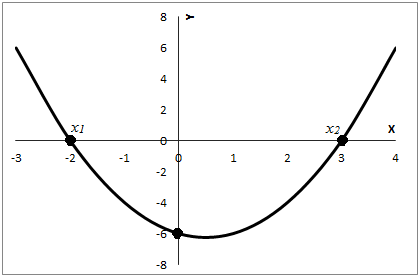
\includegraphics[width=3.57in,height=2.45in]{capitulos/funcao_do_segundo_grau/media/image5.png}
	\end{Center}
\end{figure}

Novamente incentivamos o leitor a obter o gráfico do presente exemplo em uma planilha eletrônica \qedsymbol{}
\end{texemplo}

Se $x_1 e x_2$ são raízes da equação de 2\degree grau e $A = 1$, então $0 = x$
$x_2 + Bx + C$ pode ser fatorada como

     \( 0= \left( x+a \right)  \left( x+b \right) =x^{2}+ \left( a+b \right) x+ab= x^{2}+Bx+C_{~ } \). \tab (3.4)

Assim,

 \( B=a+b _{~ } \)  e  \( C=~a \cdot  b  _{~ } \) 

Para que a Eq. (3.4) seja nula, \textit{(x+a) = (x+b) = 0}   e  \textit{a} e \textit{b} são as raízes com o sinal oposto desta equação:

 \textit{a = -x\textsubscript{1}} e \textit{b = - x\textsubscript{2} . }

Re-escrevendo a Eq. 3.4 temos:

 \( 0= \left( x-x_{1} \right)  \left( x-x_{2} \right) = x^{2}+Bx+C_{~ } \) \tab (3.5)

\begin{texemplo}
Escreva três equações do 2º grau cujas raízes sejam  \textit{x\textsubscript{1} = 2  e x\textsubscript{2} = -1}. 

\textbf{Solução}: Usando a Eq. 3.5 podemos escrever:

 \( 0= \left( x-2 \right)  \left( x+1 \right) = x^{2}-x-2_{~ } \) .

Multiplicando a equação obtida por qualquer número real, obtemos equações cuja solução é  \textit{x\textsubscript{1} = 2  e x\textsubscript{2} = -1}.   Por exemplo:

 \( 0=2x^{2}-2x-4_{~ } \)    ;       \( 0=3x^{2}-3x-6_{~ } \)    e      \( 0=4x^{2}-4x-8_{~ } \)   \qedsymbol{}
\end{texemplo}

\subsection{Vértice da parábola}

O vértice é o ponto \textit{V=(x\textsubscript{v},y\textsubscript{v})} pelo qual passa o eixo de simetria da parábola. 

\begin{figure}[H]
	\begin{Center}
		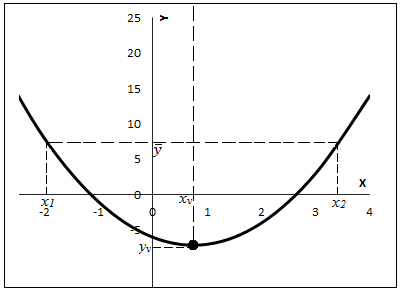
\includegraphics[width=3.15in,height=2.07in]{capitulos/funcao_do_segundo_grau/media/image6.png}
	\end{Center}
\end{figure}

Consideremos um valor  \( y \)  , tal que  \( y>y_{v} \)  , como indica a figura acima. Devido à simetria das parábolas, devem existir \textit{x\textsubscript{1}} e \textit{x\textsubscript{2}}  tal que

i) \textit{f(x\textsubscript{1}) = f(x\textsubscript{2})} =  \( y \) e

ii)    \( x_{v}=\frac{x_{1}+x_{2}}{2} \)  .    

Assim, de (i) e da Eq. 2.3, temos:

 \( y=Ax_{1}^{2}+Bx_{1}+C_{~ } \) \tab (3.6)

 \( y=Ax_{2}^{2}+Bx_{2}+C_{~ } \) \tab (3.7)

Subtraindo as Eqs. (3.6) e (3.7) e colocando \textit{A} e \textit{B} em evidência, temos:

 \( 0=A \left( x_{2}^{2}-x_{1}^{2} \right) +B \left( x_{2}-x_{1} \right) ._{~ } \) \tab (3.8)

Fatorando a diferença de dois quadrados no fator que multiplica \textit{A}, temos:

 \( 0=A \left( x_{2}+x_{1} \right)  \left( x_{2}-x_{1} \right) +B \left( x_{2}-x_{1} \right) ._{~ } \) \tab (3.9)

De (ii) temos \( 2x_{v}=x_{1}+x_{2} \) , que substituindo na Eq. (3.9)

 \( 0=A \cdot 2x_{v} \cdot  \left( x_{2}-x_{1} \right) +B \left( x_{2}-x_{1} \right) ._{~ } \)  \tab (3.10)

Dividindo a Eq. (3.10) por  \(  \left( x_{2}-x_{1} \right) _{~ } \) , pois \textit{x\textsubscript{1} $ \neq $   x\textsubscript{2}}, temos:

\[ 0=A \cdot 2x_{v}+B._{~ } \] 

E, finalmente, resolvendo para \textit{x\textsubscript{v}}, temos:

 \( x_{v}=\frac{-B}{2A}._{~ } \) \tab (3.11)

A ordenada do vértice pode ser obtida substituindo \textit{x\textsubscript{v}}  na Eq. (2.3)  

 \( y_{v}=f \left( x_{v} \right) =Ax_{v}^{2}+Bx_{v}+C_{~ } \) .

Substituindo a expressão de \textit{x\textsubscript{v}} da Eq. (3.11), tem-se: 

 \( y_{v}=f \left( x_{v} \right) =A \left( \frac{-B}{2A} \right) ^{2}+B \left( \frac{-B}{2A} \right) +C_{~ } \) \tab (3.12)

Resolvendo o quadrado, o produto e adicionando as frações, obtém-se:

 \( y_{v}=f \left( x_{v} \right) =-\frac{B^{2}-4AC}{4A}._{~ } \) \tab (3.13)

\begin{texemplo}
Faça um esboço do gráfico da função \textit{f(x) = x\textsuperscript{2} +2x+1}. 

\textbf{Solução}: Aplicando a Eq. (3.3) com \textit{A=1; B=2 }e\textit{ C=1 } obtemos duas raízes iguais   \textit{x\textsubscript{1} = }  \textit{x\textsubscript{2} = -1}. Com isto, já sabemos que a parábola tangencia o eixo \textit{X} em (-1,0). 

\begin{figure}[H]
	\begin{Center}
		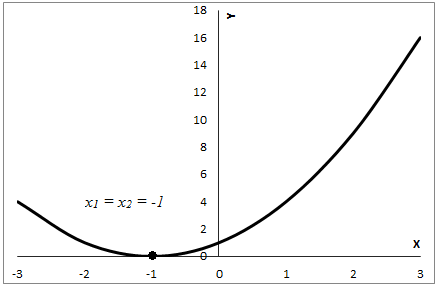
\includegraphics[width=3.26in,height=2.27in]{capitulos/funcao_do_segundo_grau/media/image7.png}
	\end{Center}
\end{figure}

Usando as Eqs. (3.11) e (3.13) encontramos o vértice: \textit{V=(-1,0)}. Com isso, sabemos que o eixo de simetria é a reta vertical  \textit{x = -1}. Como \textit{A=1 > 0} a parábola tem concavidade para cima. Com essas informações podemos traçar um esboço da parábola \qedsymbol{}
\end{texemplo}

\begin{texemplo}
Faça um esboço do gráfico da função \textit{f(x) = -x\textsuperscript{2} + 4}. 

\textbf{Solução}: Aplicando a Eq. (3.3) com \textit{A=-1; B=0 }e\textit{ C=4 } obtemos duas raízes   \textit{x\textsubscript{1} = -2} e  \textit{x\textsubscript{2} = +2}. Com isto, já sabemos que a parábola intersecta o eixo \textit{X} em (-2,0) e (2,0).

\begin{figure}[H]
	\begin{Center}
		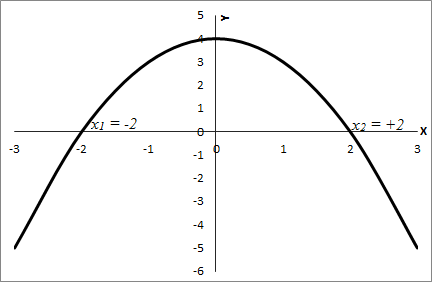
\includegraphics[width=3.18in,height=2.19in]{capitulos/funcao_do_segundo_grau/media/image8.png}
	\end{Center}
\end{figure}

Usando as Eqs. (3.11) e (3.13) encontramos o vértice: \textit{V=(0,4)}. Com isso, sabemos que o eixo de simetria é o próprio eixo \textit{Y}. Como \textit{A=-1 < 0} a parábola tem concavidade para baixo. Com essas informações podemos traçar um esboço da parábola \qedsymbol{}
\end{texemplo}

\begin{texemplo}
Faça um esboço do gráfico da função \textit{f(x) = x\textsuperscript{2} +1}. 

\textbf{Solução}: Aplicando a Eq. (3.3) com \textit{A=1; B=0 }e\textit{ C=1 } obtemos discriminante negativo, portanto as raízes não são reais. Temos outras informações para fazer um esboço do gráfico:

Usando as Eqs. (3.11) e (3.13) encontramos o vértice: \textit{V=(0,1)}. Com isso, sabemos que o eixo de simetria é o próprio eixo \textit{Y}. A parábola intersecta \textit{Y} em (\textit{0,1}).

Como \textit{A=1 > 0} a parábola tem concavidade para cima. Usaremos os pontos (\textit{1,2}) e (-\textit{1,2}) apenas para ter uma ideia da concavidade. Com essas informações podemos traçar um esboço da parábola\qedsymbol{}

\begin{figure}[H]
	\begin{Center}
		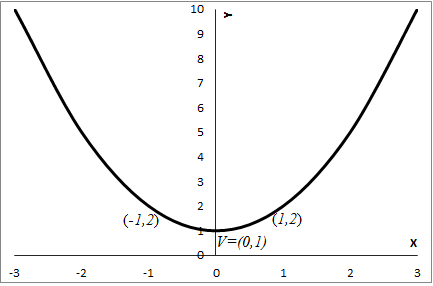
\includegraphics[width=3.44in,height=2.23in]{capitulos/funcao_do_segundo_grau/media/image9.png}
	\end{Center}
\end{figure}
\end{texemplo}

\subsection{Parábolas com eixo de simetria paralelos a X}

As parábolas com eixo de simetria paralelos a \textit{X}   \textbf{NÃO SÃO FUNÇÕES}, pois para cada \textit{x} temos dois valores de \textit{y}.

As expressões das parábolas com eixo de simetria paralelos a \textit{X} são obtidas trocando as variáveis \textit{x} e \textit{y} na Eq. (2.3):

 \( x=Ay^{2}+By+C_{~ } \) . \tab (3.14)

Se na Eq. (3.14) \textit{B = 0},  a parábola tem o eixo de simetria sobre o eixo X e sua equação é

 \( x=Ay^{2}+C_{~ } \)        ou       \( y= \pm \sqrt[]{\frac{x-C}{A}}_{~ } \)  \tab (3.15)

Se na Eq. (3.14) \textit{B = 0} e \textit{C = 0}   a parábola tem o eixo de simetria sobre o eixo X, o vértice na origem e sua equação é

 \( x=Ay^{2}_{~ } \)        ou       \( y= \pm \sqrt[]{\frac{x}{A}}_{~ } \)  \tab (3.16)

\begin{texemplo}
Faça um esboço do gráfico da parábola \textit{ x = y\textsuperscript{2} - 1}. 

\textbf{Solução}: Observe que para \textit{y = $ \pm $  2}, obtém-se o mesmo valor de \textit{x = 3}.  Portanto esta parábola não é uma função.

Usando as informações sobre raízes e vértices, temos:

\begin{figure}[H]
	\begin{Center}
		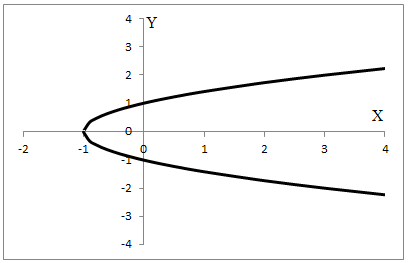
\includegraphics[width=3.62in,height=2.74in]{capitulos/funcao_do_segundo_grau/media/image10.png}
	\end{Center}
\end{figure}

Raízes: \textit{y\textsubscript{1} = 1}   e  \textit{y\textsubscript{2} = -1}   e   vértice: \textit{V=(0,-1)}. Como \textit{A=1 > 0} a concavidade é para a direita \qedsymbol{}
\end{texemplo}

\begin{texemplo}
Faça um esboço do gráfico da parábola \textit{ x = - y\textsuperscript{2} + 4}. 

\textbf{Solução}:  Usando as informações sobre raízes e vértices, temos:

\begin{figure}[H]
	\begin{Center}
		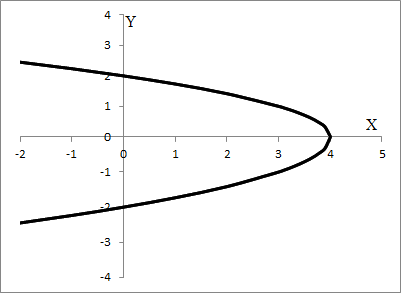
\includegraphics[width=3.43in,height=2.43in]{capitulos/funcao_do_segundo_grau/media/image11.png}
	\end{Center}
\end{figure}

Raízes: \textit{y\textsubscript{1} = 2}   e  \textit{y\textsubscript{2} = -2}   e   vértice: \textit{V=(0,4)}. Como \textit{A=-1 < 0} a concavidade é para a esquerda \qedsymbol{}
\end{texemplo}

\section{Sinal da função do 2º grau}

Lembremos que o sinal da função \textit{y=f(x)} é o sinal da variável \textit{y} em cada ponto. As raízes e a concavidade das parábolas são os elementos necessários para determinar o sinal da função. 

Seja   \textit{f(x) = Ax\textsuperscript{2} +Bx +C}, vamos analisar três casos:

\textbf{Caso 1}: \textbf{\textit{f(x)} não tem raízes reais}.  

Então \textit{f(x)} não intercepta o eixo \textit{X}. 

Nesse caso, \textit{$ \Delta $  = B\textsuperscript{2} - 4AC < 0   }e\textit{:  }

Se \textit{A > 0} ,   \textit{f(x)} é POSITIVA para qualquer \textit{x   ;}

Se \textit{A < 0} ,   \textit{f(x)} é NEGATIVA para qualquer \textit{x   ;}

\begin{figure}[H]
	\begin{Center}
		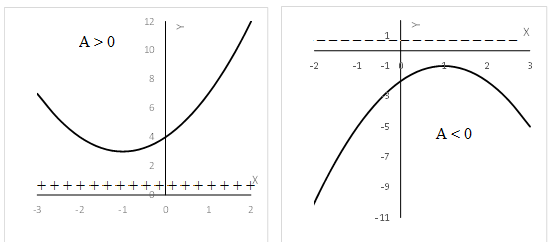
\includegraphics[width=5.74in,height=2.52in]{capitulos/funcao_do_segundo_grau/media/image12.png}
	\end{Center}
\end{figure}

\textbf{Caso 2}: \textbf{\textit{f(x)}  tem raízes reais idênticas}.  (\textit{x\textsubscript{1} = x\textsubscript{2} )}   

Então \textit{f(x)}  tangencia o eixo \textit{X} em um ponto: (\textit{x\textsubscript{1} , 0)}   

Nesse caso, \textit{$ \Delta $  = B\textsuperscript{2} - 4AC = 0   }e\textit{:  }

Se \textit{A > 0} ,   \textit{f(x)} é POSITIVA para qualquer \textit{x   , / x $ \neq $  x\textsubscript{1};}

Se \textit{A < 0} ,   \textit{f(x)} é NEGATIVA para qualquer \textit{x   , / x $ \neq $  x\textsubscript{1  }}e

Para \textit{x $ \neq $  x\textsubscript{1}   f(x) = 0.}

\begin{figure}[H]
	\begin{Center}
		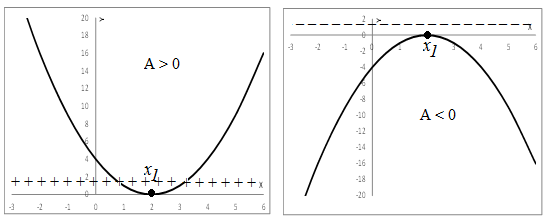
\includegraphics[width=5.67in,height=2.32in]{capitulos/funcao_do_segundo_grau/media/image13.png}
	\end{Center}
\end{figure}

\textbf{Caso 3}: \textbf{\textit{f(x)}  tem raízes reais distintas}.  (\textit{x\textsubscript{1} $ \neq $  x\textsubscript{2} )}   

Então \textit{f(x)}  intersecta o eixo \textit{X} em dois pontos: (\textit{x\textsubscript{1} , 0)}   e  (\textit{x\textsubscript{2} , 0).}   

Nesse caso, \textit{$ \Delta $  = B\textsuperscript{2} - 4AC > 0   }e\textit{:  }

Se \textit{A > 0} ,   \textit{f(x)} é POSITIVA para qualquer \textit{x   , / x < x\textsubscript{1  }}ou\textit{ x > x\textsubscript{2  }}e

\textit{f(x)} é NEGATIVA para qualquer \textit{x   , / x\textsubscript{1  }< x < x\textsubscript{2  }}.

Se \textit{A < 0} ,   \textit{f(x)} é POSITIVA para qualquer \textit{x   , / x\textsubscript{1  }< x < x\textsubscript{2  }}e

\textit{f(x)} é NEGATIVA para qualquer \textit{x   , x < x\textsubscript{1  }}ou\textit{ x > x\textsubscript{2  . }}

\begin{figure}[H]
	\begin{Center}
		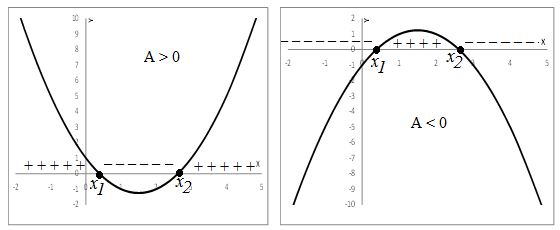
\includegraphics[width=5.83in,height=2.4in]{capitulos/funcao_do_segundo_grau/media/image14.png}
	\end{Center}
\end{figure}

\begin{texemplo}
Determine os sinais e faça um esboço do gráfico da função

 \textit{f(x) = -x\textsuperscript{2} +x -1}. 

\textbf{Solução}: O discriminante \textit{$ \Delta $  = -3 < 0  }e o\textit{ A=-1 < 0. }Portanto, trata-se do Caso 1\textit{: f(x) }é NEGATIVA para qualquer \textit{x} real\qedsymbol{}

\begin{figure}[H]
	\begin{Center}
		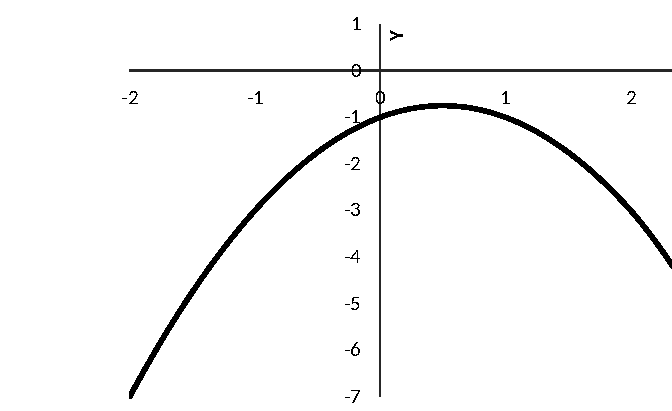
\includegraphics[width=3.55in,height=2.2in]{capitulos/funcao_do_segundo_grau/media/image15.pdf}
	\end{Center}
\end{figure}
\end{texemplo}

\begin{texemplo}
Determine os sinais e faça um esboço do gráfico da função

 \textit{f(x) = x\textsuperscript{2} - x }. 

\textbf{Solução}: O discriminante \textit{$ \Delta $  = 1> 0}. As raízes são   \textit{x\textsubscript{1}} = 0 e \textit{ x\textsubscript{2} = 1} então trata-se do Caso 3\textit{. }Como \textit{A = 1 > 0},, tem-se:

\textit{f(x)} será  POSITIVA se \textit{x < 0}  ou   \textit{x > 1    }e  NEGATIVA    se    \textit{0  <  x  <  1}\qedsymbol{}

\begin{figure}[H]
	\begin{Center}
		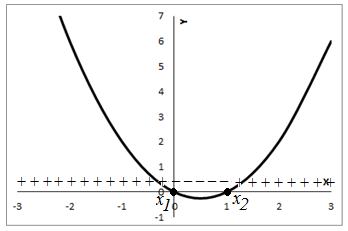
\includegraphics[width=3.62in,height=2.41in]{capitulos/funcao_do_segundo_grau/media/image16.png}
	\end{Center}
\end{figure}
\end{texemplo}

\section{Pontos de máximo e de mínimo}

\begin{caixa}
O vértice (\textit{V}) é um ponto de máximo ou de mínimo das parábolas.

Se \textit{A >  0} então \textit{V} é de \textbf{mínimo}, 

Se \textit{A <  0} então \textit{V} é de \textbf{máximo}. 
\end{caixa}

\begin{texemplo}
Encontre o ponto de máximo da função:  \textit{f(x) = -x\textsuperscript{2} - 4x +8}. 

\textbf{Solução}: Para determinar as coordenadas do vértice usamos as Eqs. 3.11 e 3.13:

 \( x_{v}=\frac{- \left( -4 \right) }{2 \left( -1 \right) }=-2_{} \)      e        \( y_{v}=-\frac{ \left( -4 \right) ^{2}-4 \left( -1 \right)  \left( 8 \right) }{4 \left( -1 \right) }=12._{~ } \) 

O maior valor (ponto máximo) de  \textit{f(x) } ocorre em \textit{x = -2} e é \textit{y = 12} \qedsymbol{}
\end{texemplo}

\begin{texemplo}
Em um experimento de cultivo de beterraba foram obtidos os dados da tabela para (\textit{x}) número de mudas/\textit{m\textsuperscript{2}} e (\textit{P}) produtividade (\textit{kg/m\textsuperscript{2}}).

\begin{table}[H]
 			\centering
\begin{tabular}{p{1.68in}p{0.38in}p{0.39in}}
\hline
%row no:1
\multicolumn{1}{|p{1.68in}}{\textit{x}, nº de mudas/\textit{m\textsuperscript{2} (unid)}} & 
\multicolumn{1}{|p{0.38in}}{20} & 
\multicolumn{1}{|p{0.39in}|}{50} \\
\hhline{---}
%row no:2
\multicolumn{1}{|p{1.68in}}{\textit{P}, produtividade (kg/\textit{ m\textsuperscript{2})}} & 
\multicolumn{1}{|p{0.38in}}{0,8} & 
\multicolumn{1}{|p{0.39in}|}{0,6} \\
\hhline{---}

\end{tabular}
 \end{table}

É razoável considerar que para nenhuma muda plantada (\textit{x=0}) a produtividade é nula (\textit{P=0}). 

	a) Determine uma função do segundo grau para descrever a relação entre \textit{P} e \textit{x}.

	b) Calcule o número de mudas que levaria a produtividade máxima.

\textbf{Solução}: a) O coeficiente \textit{C}  de \textit{P(x)= Ax\textsuperscript{2} + Bx + C } é zero, pois a parábola intersecta em \textit{P = 0}.

Substituindo os valores de \textit{x} e \textit{P} na equação   \textit{P(x) = Ax\textsuperscript{2} + Bx }obtemos um sistema de duas equações com duas variáveis, \textit{A} e \textit{B}:

\textit{0,8 = 400A  + 20B}

\textit{0,6 = 2500A + 50B}

Resolvendo o sistema obtemos:\textit{ A = -0,00093  }e \textit{ B = 0,0586. }

A função produtividade é:  \textit{P(x) = -0,00093  x\textsuperscript{2} + 0,0586x.}

\begin{figure}[H]
	\begin{Center}
		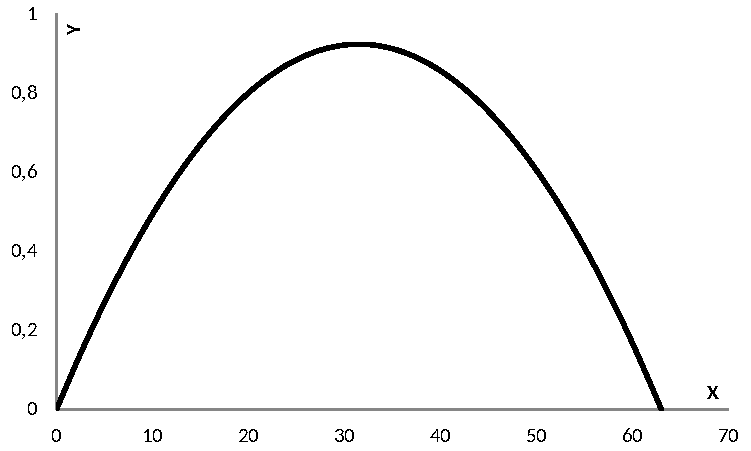
\includegraphics[width=3.46in,height=2.26in]{capitulos/funcao_do_segundo_grau/media/image17.pdf}
	\end{Center}
\end{figure}

	b) A produtividade máxima será no vértice de\textit{ P(x). }Usando as Eqs. (3.11) e (3.13) obtemos\textit{ : x\textsubscript{v} = 31,42 mudas/m\textsuperscript{2} }e\textit{  P\textsubscript{v} =0.92 kg }\qedsymbol{}
\end{texemplo}

\section{Aplicações das funções quadráticas}

As funções quadráticas são utilizadas em alguns fenômenos físicos e em como função de ajuste em problemas de otimização. Vamos analisar alguns desses casos.

\subsection{Queda livre}

O movimento vertical de uma pedra, tanto de subida como de descida, desconsiderando a presença do ar, pode ser modelado por uma função quadrática. 

 \( y \left( t \right) =y_{o}+v_{o}t-\frac{1}{2}gt^{2}~  \) \tab (6.1)

onde \textit{y(t)  é a posição no eixo Y vertical, apontando para cima (m), }

\textit{ y\textsubscript{o  é a posição inicial (m), }}

\textit{v\textsubscript{o  é a velocidade inicial (m/s), }}

\textit{g é a aceleração da gravidade (m/s\textsuperscript{2) e }}

\textit{t é o tempo (s).}

A velocidade da pedra em cada instante, é dada por uma função de 1º grau:

 \( v \left( t \right) =v_{o}-gt~~~  \) \tab (6.2)

\begin{figure}[H]
	\begin{Center}
		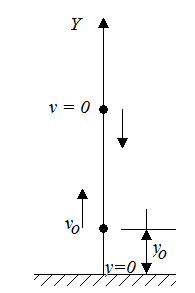
\includegraphics[width=2.03in,height=3.05in]{capitulos/funcao_do_segundo_grau/media/image18.png}
	\end{Center}
\end{figure}

Consideremos que \textit{y = 0 corresponde ao nível do chão. Se uma pedra é jogada para cima por uma pessoa em pé, a posição de saída é  y\textsubscript{o  e como a pedra está recebendo um impulso, a velocidade inicial é vo , diferente de zero, e com sinal positivo, pois o deslocamento é para cima, sentido positivo do eixo Y.  A aceleração da gravidade g é constante para pequenas variações de altitude. A Eq. (6.1) dá as posições da pedra para cada instante de tempo.}}

\begin{enumerate}
	\item Considere \textit{y\textsubscript{o} = 1 m; v\textsubscript{o}=+5 m/s }e\textit{ g= 10 m/s\textsuperscript{2}} e faça um gráfico de  \textit{y(t)  .}

	\item Determine a altura máxima que a pedra alcançará e o tempo correspondente a esta posição, usando o que você conhece sobre vértice de parábolas.

	\item A velocidade da pedra na posição de altura máxima é zero. Use a Eq. (6.2) para calcular o tempo que a pedra levará para atingir a altura máxima. Compare o resultado com o item (b).

	\item Analise o sinal da velocidade em função do tempo.

	\item Calcule o tempo que a pedra levará para atingir o chão.

	\item Calcule a velocidade da pedra ao atingir o chão.
\end{enumerate}

\subsection{Arcos parabólicos em construções}

\begin{multicols}{2}
    Os arcos parabólicos são utilizados em construções, principalmente em portas, janelas, pontes e aquedutos. Consegue-se maior resistência em estruturas na forma de arcos, para grandes vãos, do que com vigas retas. 

\begin{minipage}{0.5\columnwidth}
\centering
    \fbox{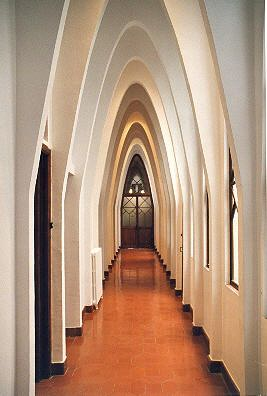
\includegraphics[width=\dimexpr\textwidth-2\fboxsep-2\fboxrule\relax]{capitulos/funcao_do_segundo_grau/media/image19.png}}
\end{minipage}%
\begin{minipage}{0.5\columnwidth}
\centering
    \fbox{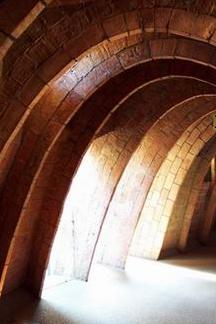
\includegraphics[width=\dimexpr\textwidth-2\fboxsep-2\fboxrule\relax]{capitulos/funcao_do_segundo_grau/media/image20.png}}
    \end{minipage}
\end{multicols}

Consideremos a construção de uma janela composta por um retângulo e uma parábola na parte superior, conforme mostra a figura.

\begin{figure}[H]
	\begin{Center}
		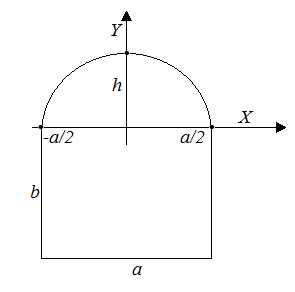
\includegraphics[width=2.16in,height=2.09in]{capitulos/funcao_do_segundo_grau/media/image21.png}
	\end{Center}
\end{figure}

Podemos determinar uma equação de 2º grau para modelar o arco. Sejam \textit{x\textsubscript{1}= a/2} e \textit{x\textsubscript{2  }=-a/2} as raízes da parábola.

Reescrevendo a Eq. (3.5) multiplicada por \textit{A} (coeficiente de \textit{x\textsuperscript{2}}, na Eq. 2.3), temos:

 \( F \left( x \right) =A \left( x-x_{1} \right)  \left( x-x_{2} \right) ~~ ^{}_{~ } \) \tab (6.3)

 Substituindo as raízes na Eq.(6.3) temos

    \( F \left( x \right) =A \left( x-\frac{a}{2} \right)  \left( x+\frac{a}{2} \right) =A \left( x^{2}-\frac{a^{2}}{4} \right) ~ ^{}_{~ } \) .\tab \tab \tab (6.4)

Substituindo as coordenadas do vértice \textit{V=(0,h)}  na Eq. ( 6.4), temos

 \( h=-A\frac{a^{2}}{4}~~ ^{}_{~ } \).

Então \( A=-\frac{4h}{a^{2}}~~ ^{}_{~ } \) .

Substituindo esta expressão de \textit{A} na Eq. (6.4), temos

 \( F \left( x \right) =\frac{h}{a^{2}} \left( a^{2}-4x^{2} \right) ~ ^{}_{~ } \) .

	a) Considerando \textit{a = 1,6 m} e \textit{h  = 0,6 m}, determine a função \textit{F(x)}.

	b) Use a função \textit{F(x)} para determinar ao menos cinco pontos para \textit{0 < x < a/2}, que poderiam ser utilizados para fazer a forma de madeira, sobre a qual são assentados os tijolos.

\subsection{Problemas de otimização (dados de experimentos)}

Em experimentos de cultivos de espécies é comum obter-se dados de (\textit{P}) produtividade por outra variável (\textit{x}) tal como o número de mudas, a quantidade de um fertilizante ou de água. Neste tipo de problema, o objetivo é determinar o valor de \textit{x} que \textbf{maximiza} a produtividade. 

Se o número de dados disponíveis é de apenas três pontos, existe uma única parábola que passa por eles. Para determinar a parábola, podemos substituir os valores (\textit{x\textsubscript{i},P\textsubscript{i}}) na função de 2º grau

\textit{P(x)= Ax\textsuperscript{2} + Bx + C }. \tab (6.5)

\begin{table}[H]
 			\centering
\begin{tabular}{p{0.71in}p{0.71in}p{0.71in}p{0.71in}}
\hline
%row no:1
\multicolumn{1}{|p{0.71in}}{\textit{x}} & 
\multicolumn{1}{|p{0.71in}}{\textit{x\textsubscript{1}}} & 
\multicolumn{1}{|p{0.71in}}{\textit{x\textsubscript{2}}} & 
\multicolumn{1}{|p{0.71in}|}{\textit{x\textsubscript{3}}} \\
\hhline{----}
%row no:2
\multicolumn{1}{|p{0.71in}}{\textit{P}} & 
\multicolumn{1}{|p{0.71in}}{\textit{P\textsubscript{1}}} & 
\multicolumn{1}{|p{0.71in}}{\textit{P\textsubscript{2}}} & 
\multicolumn{1}{|p{0.71in}|}{\textit{P\textsubscript{3}}} \\
\hhline{----}

\end{tabular}
 \end{table}

Obtemos um sistema linear de três equações e três incógnitas:

\begin{multicols}{2}
 \(  \left\{ \begin{matrix}
P_{1}=Ax_{1}^{2}+Bx_{1}+C\\
P_{2}=Ax_{2}^{2}+Bx_{2}+C\\
P_{3}=Ax_{3}^{2}+Bx_{3}+C\\
\end{matrix} \right\} \)

(6.6)
\end{multicols}

A solução do sistema Eq. (6.6) pode ser obtida pelo Método de Cramer (determinantes). A matriz dos coeficientes e a dos termos independentes são:

 \( M= \left[ \begin{matrix}
x_{1}^{2}  &  x_{1}  &  1\\
x_{2}^{2}  &  x_{2}  &  1\\
x_{3}^{2}  &  x_{3}  &  1\\
\end{matrix}
 \right]  \)        e       \( b= \left[ \begin{matrix}
P_{1}\\
P_{2}\\
P_{3}\\
\end{matrix}
 \right]  \) 

Por este método, são construídas três matrizes, substituindo o vetor b em cada coluna da matriz A.

 \( M_{1}= \left[ \begin{matrix}
P_{1}  &  x_{1}  &  1\\
P_{2}  &  x_{2}  &  1\\
P_{3}  &  x_{3}  &  1\\
\end{matrix}
 \right]  \) ;             \( M_{2}= \left[ \begin{matrix}
x_{1}^{2}  &  P_{1}  &  1\\
x_{2}^{2}  &  P_{2}  &  1\\
x_{3}^{2}  &  P_{3}  &  1\\
\end{matrix}
 \right]  \)           e          \( M_{3}= \left[ \begin{matrix}
x_{1}^{2}  &  x_{1}  &  P_{1}\\
x_{2}^{2}  &  x_{2}  &  P_{2}\\
x_{3}^{2}  &  x_{3}  &  P_{3}\\
\end{matrix}
 \right]  \) 

Os determinantes das matrizes \textit{M, M\textsubscript{1}},  \textit{M\textsubscript{2}} e \textit{M\textsubscript{3}}  são obtidos pela Regra de Sarrus e a solução pelas razões:

 \( A=\frac{det \left( M_{1} \right) }{det \left( M \right) } \), \( B=\frac{det \left( M_{2} \right) }{det \left( M \right) } \) e \( C=\frac{det \left( M_{3} \right) }{det \left( M \right) } \) .

Levando os valores de \textit{A, B} e \textit{C} na Eq. (6.5) obtém-se a função que passa nos três pontos dados. 

O cálculo de \textit{x} que corresponde à maior produtividade é o cálculo das coordenadas do vértice da parábola.

Os dados da tabela abaixo são de um experimento com beterraba.

\begin{table}[H]
 			\centering
\begin{tabular}{p{1.68in}p{0.38in}p{0.39in}p{0.39in}}
\hline
%row no:1
\multicolumn{1}{|p{1.68in}}{\textit{x}, nº de mudas/\textit{m\textsuperscript{2} (unid)}} & 
\multicolumn{1}{|p{0.38in}}{20} & 
\multicolumn{1}{|p{0.39in}}{30} & 
\multicolumn{1}{|p{0.39in}|}{50} \\
\hhline{----}
%row no:2
\multicolumn{1}{|p{1.68in}}{\textit{P}, produtividade (kg/\textit{ m\textsuperscript{2})}} & 
\multicolumn{1}{|p{0.38in}}{0,8} & 
\multicolumn{1}{|p{0.39in}}{1,2} & 
\multicolumn{1}{|p{0.39in}|}{0,6} \\
\hhline{----}

\end{tabular}
 \end{table}

	a) Determine uma função do segundo grau para descrever a relação entre \textit{P} e \textit{x}.

	b) Calcule o número de mudas que levaria a produtividade máxima.

\subsection{Antena parabólica}

Consideremos uma parábola. Se a girarmos em torno de seu eixo, obteremos uma superfície chamada paraboloide de revolução. Uma antena parabólica é um paraboloide de revolução. Porque as antenas têm esta forma geométrica?

As parábolas têm um ponto característico chamado \textit{foco com a seguinte propriedade: toda reta paralela ao eixo, reflete passando pelo foco. No caso das antenas, as radiações eletromagnéticas vindas do espaço em múltiplas direções. Aquelas que são paralelas ao eixo de simetria da antena, são concentradas no foco, onde está o captador e assim o sinal é concentrado, melhorando a qualidade da recepção.}

\begin{figure}[H]
	\begin{Center}
		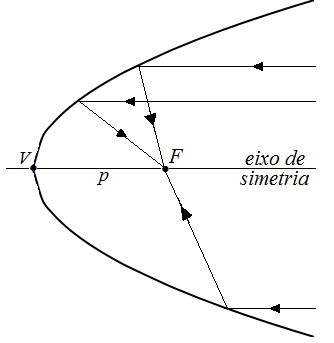
\includegraphics[width=2.15in,height=2.0in]{capitulos/funcao_do_segundo_grau/media/image22.png}
	\end{Center}
\end{figure}

A equação canônica de uma parábola com eixo de simetria horizontal é

$y^2$ = $4Fx$, \tab (6.7)

onde \textit{F é a distância do vértice ao foco. Com essas informações, podemos construir parábolas com o foco conhecido. Por exemplo, se  F = 0,5 m, podemos encontrar os pontos da parábola, atribuindo valores de x e calculando os de y, através da Eq. (6.7).}

 \( ~ y=  \pm \sqrt[]{2x} \). \tab (6.8)

Assim, para \textit{x = 0,6 cm (diâmetro de 1,2 m) teremos y = 1,095m (altura \textbf{d na figura).}}

\begin{figure}[H]
	\begin{Center}
		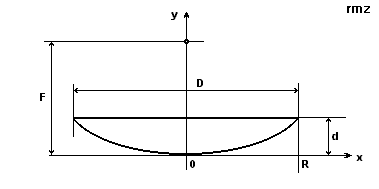
\includegraphics[width=3.95in,height=1.97in]{capitulos/funcao_do_segundo_grau/media/image23.png}
	\end{Center}
\end{figure}

	a) Calcule a posição \textit{F} do foco, se \textit{d = 0,8m}  e o diâmetro da antena é \textit{1 m}. 

	b) Meça o diâmetro e a altura \textbf{d} de uma antena parabólica real e calcule o foco \textit{F}. Verifique se esta localização coincide com a posição do coletor de radiação eletromagnética do equipamento.

\section{Exercícios}
\begin{enumerate}[label=\thechapter.\arabic*]
\exitem{} Considere que o lado de um quadrado é expresso pela variável \textit{x}.

a) Escreva a função que expressa a área \textit{A do quadrado em função do lado x.}

b) Faça uma tabela com valores de \textit{x e A.}

c) Faça um gráfico da função \textit{A(x).}

d) A dependência entre \textit{A e x é linear ? }

\exitem{} Considere que o lado de um quadrado é expresso pela função \textit{x+1}.

a) Escreva a função que expressa a área \textit{A do quadrado em função da variável x.}

b) Faça um gráfico da função \textit{A(x) e compare com o gráfico do Ex. 1.}

\exitem{} Nos Exs. 1 e 2 a função área \textit{A(x)} tem sentido para \textit{x $ \leq $  0} ?

\exitem{} Determine a função que expressa a área de cada figura.

\begin{figure}[H]
	\begin{Center}
		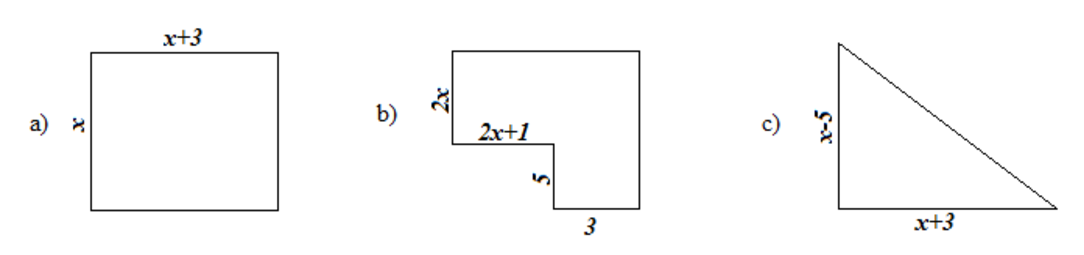
\includegraphics[width=5.91in,height=1.39in]{capitulos/funcao_do_segundo_grau/media/image24.pdf}
	\end{Center}
\end{figure}

\exitem{} Nas funções abaixo: calcule as raízes, identifique os pontos de intersecção com os eixos coordenados, calcule o vértice e faça o gráfico:

a) $f(x) = x^2 - 1$

b) f(x) = $x^2 -2x - 3$

c) $f(x) =- x^2 - x + 6$

d) $f(x) = x^2 + 2x - 8$

\exitem{} Identifique os intervalos em que cada função do Ex. 5, é positiva ou negativa. (Faça um desenho do eixo X indicando o sinal da função).

\exitem{} A área de um círculo é dada pela fórmula:  \textit{A = $ \pi $  r\textsuperscript{2}}, onde \textit{r} é o raio. Faça um gráfico da função \textit{A(r),} para \textit{r < 4 cm}.

\exitem{} O deslocamento de uma pedra em queda livre (sem o atrito do ar e influência do vento) é dato pela fórmula:  \textit{y(t) = y\textsubscript{o} + v\textsubscript{o}t - 0,5gt\textsuperscript{2}}, onde \textit{y }é a posição no eixo \textit{Y} vertical, apontando para baixo, \textit{y\textsubscript{o}}  é a posição inicial (\textit{m}), \textit{v\textsubscript{o}}  é a velocidade inicial (m/s), \textit{g} é a aceleração da gravidade (\textit{m/s\textsuperscript{2}}) e \textit{t} é o tempo (\textit{s}). 

\begin{enumerate}[label=\thechapter.\alph*)]
	\item Escreva a função \textit{y(t) }sabendo que:   \textit{ y\textsubscript{o} = 1 m; v\textsubscript{o}=10 m/s }e\textit{ g= 9,8 m/s\textsuperscript{2}.}

	\item Faça um gráfico de   \textit{y(t)}

	\item Calcule o tempo para que a pedra atinja a altura máxima

	\item Calcule a altura máxima

	\item Calcule o tempo para que a pedra atinja o chão.
\end{enumerate}

\exitem{} Escreva uma função de 2\textsuperscript{o} grau cujas raízes são: 

a) $x_1 = 2$ e $x_2 = 3$

c) $x_1 = -2$ e $x_2 = 1$

b) $x_1 = 3$ e $x_2 = 4$

d) $x_1 = -3$ e $x_2 = 2$

\exitem{} Faça um esboço do gráfico das funções do 2o grau usando as informações disponíveis.

a) As raízes são $x_1 = 1$ e $x_2 = 3$ ; o vértice é $V=(2,-2)$

b) As raízes são $x_1 = 1$ e $x_2 = 3$ ; o vértice é $V=(2,2)$

c) As raízes são $x_1 = 1$ e $x_2 = -1$ ; e a função intersecta $Y$ em $(0,1)$

d) A função intercecta X em $x_1 = 0$ e $x_2 = 2$ ; e o vértice é $V=(1,-2)$

\exitem{} Escreva a função de 2\textsuperscript{o} grau usando as seguintes informações:

a) O $x$ do vértice é $1$; a função intercecta $Y$ na origem; $A = -1$

b) As raízes são $x_1 = 1$ e $x_2 = 3$ e a função intersecta Y em $(0,3)$

c) As raízes são $x_1 = 1$ e $x_2 = 3$ e a função intersecta Y em $(0,6)$

d) As raízes são $x_1 = -2$ e $x_2 = 2$ e a função intersecta Y em $(0,5)$

\exitem{} Faça um esboço do gráfico das parábolas:

\begin{multicols}{4}
a) $y^2 = x + 5$

b) $y^2 = 3x - 1$

c) $y^2 = -x + 2$

d) \( y= \pm \sqrt[]{x-3} \)

e) \( y=\sqrt[]{x-2} \)

f) \( y=-\sqrt[]{x-2} \)

g) $x = y^2 - y - 2$

h) $x = -y^2 + y + 2$
\end{multicols}

\exitem{} Uma porta de casa colonial tem a forma de uma parábola com a concavidade para baixo. A altura máxima, no eixo central da porta, tem \textit{2,50 m} e a base \textit{2 m}. Para marcar o contorno da porta os pedreiros precisam alguns pontos (\textit{x,y}) para fazer a forma e assentar os tijolos, formando o arco parabólico. 

a) Determine a equação da parábola que satisfaz as medidas da porta.

b) Faça uma tabela com valores de \textit{x e y para, ao menos, cinco pontos da parábola.}

c) Faça o gráfico da parábola e indique a posição dos pontos do item (b).

\exitem{} Considere uma janela na forma de um quadrado com um semicírculo sobre ele. Encontre as dimensões da janela se a área total do quadrado e do semicírculo é  \textit{60,96m\textsuperscript{2}}.

\exitem{} Em um experimento de cultivo de cenouras foi obtida uma função que relaciona a quantidade de adubo orgânico de galinha (\textit{x, kg}) com a produtividade (\textit{P}, \textit{kg/m\textsuperscript{2}}):

\textit{P(x) = -2,13 x\textsuperscript{2} + 5,2 x -0,066.}

a) Determine a quantidade de adubo para a maior produtividade

b) Faça o gráfico de \textit{P(x) }indicando o ponto de maior produtividade.

\exitem{} Um refletor parabólico (paraboloide de revolução) tem uma lâmpada localizada no foco \textit{F = 5 cm}, com a luz direcionada para o arco parabólico, como indica a figura. Qual deve ser o diâmetro \textit{D} para que a profundidade do arco seja \textit{h = 5 cm} ? (Veja a aplicação 6.4)

\begin{figure}[H]
	\begin{Center}
		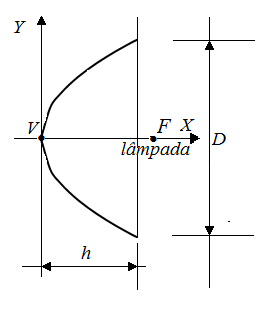
\includegraphics[width=1.85in,height=1.9in]{capitulos/funcao_do_segundo_grau/media/image25.png}
	\end{Center}
\end{figure}
\end{enumerate}

\section{RESPOSTAS DOS EXERCÍCIOS PROPOSTOS}

\begin{enumerate}[label=\thechapter.\arabic*]
\ansitem{} a)  \( A=x^{2} \) 

b)

\begin{table}[H]
\begin{Center}
\begin{tabular}{p{0.27in}p{0.29in}}
\hline
%row no:1
\multicolumn{1}{|p{0.27in}}{X} & 
\multicolumn{1}{|p{0.29in}|}{A} \\
\hhline{--}
%row no:2
\multicolumn{1}{|p{0.27in}}{0} & 
\multicolumn{1}{|p{0.29in}|}{0} \\
\hhline{--}
%row no:3
\multicolumn{1}{|p{0.27in}}{1} & 
\multicolumn{1}{|p{0.29in}|}{1} \\
\hhline{--}
%row no:4
\multicolumn{1}{|p{0.27in}}{2} & 
\multicolumn{1}{|p{0.29in}|}{4} \\
\hhline{--}
%row no:5
\multicolumn{1}{|p{0.27in}}{3} & 
\multicolumn{1}{|p{0.29in}|}{9} \\
\hhline{--}
\end{tabular}
\end{Center}
\end{table}

c)

\begin{figure}[H]
    \begin{Center}
    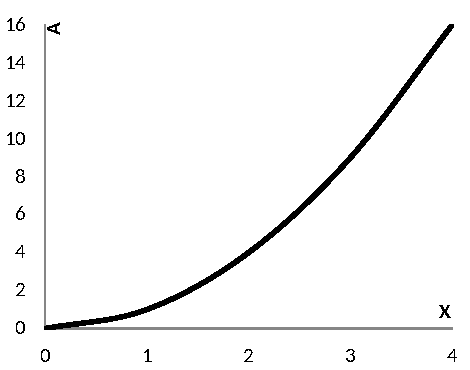
\includegraphics[width=2.18in,height=1.9in]{capitulos/funcao_do_segundo_grau/media/image26.pdf}
    \end{Center}
\end{figure}

d) Não, a dependência entre \textit{A} e \textit{x} é de 2º Grau.

\ansitem{} a)  \( A=x^{2}+2x+1 \) 

b)

\begin{figure}[H]
	\begin{Center}
		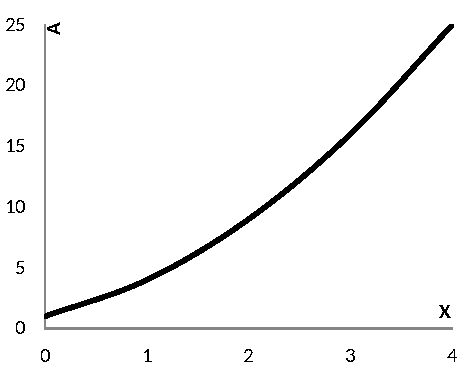
\includegraphics[width=2.16in,height=1.64in]{capitulos/funcao_do_segundo_grau/media/image27.pdf}
	\end{Center}
\end{figure}

\ansitem{} No Ex. 1.1 $A(x)=x^{2} > 0$ para qualquer \textit{x,} se \textit{x < 0} não existe quadrado. Analogamente, no Ex1.2.  para  x > -1. 

\ansitem{} a) \textit{A=x\textsuperscript{2}+3x}

b) \textit{A=x\textsuperscript{2}+8x+15}

c)  \( A=\frac{x^{2}-2x-15}{2} \) 

\ansitem{}
\begin{multicols}{2}
a) Raízes: \textit{x\textsubscript{1}=-1; x\textsubscript{2}=1}. Intersecção com Y em (0,-1); Intersecção com X em (-1,0) e (1,0); V=(0,-1)

\begin{figure}[H]
	\begin{Center}
		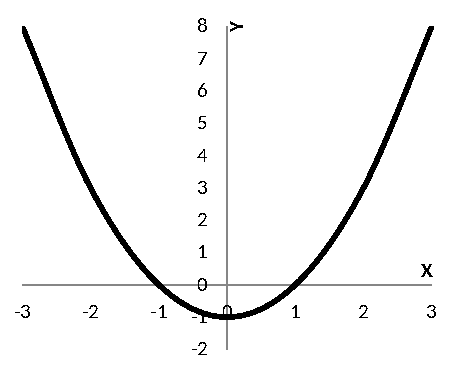
\includegraphics[width=2.15in,height=1.55in]{capitulos/funcao_do_segundo_grau/media/image28.pdf}
	\end{Center}
\end{figure}
\end{multicols}

\begin{multicols}{2}
b) Raízes: \textit{x\textsubscript{1}=-1; x\textsubscript{2}=3}. Intersecção com Y em (0,-3); Intersecção com X em (-1,0) e (3,0); V=(1,-4)

\begin{figure}[H]
	\begin{Center}
		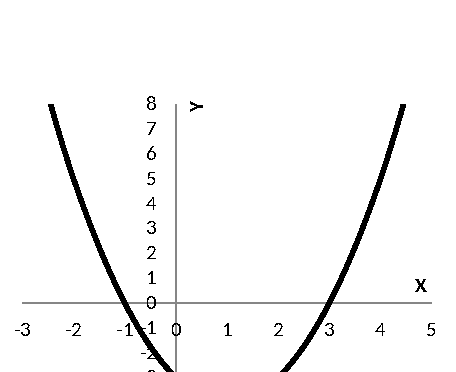
\includegraphics[width=2.15in,height=1.58in]{capitulos/funcao_do_segundo_grau/media/image29.pdf}
	\end{Center}
\end{figure}
\end{multicols}

\begin{multicols}{2}
c) Raízes: \textit{x\textsubscript{1}=-3; x\textsubscript{2}=2}. Intersecção com Y em (0,6); Intersecção com X em (-3,0) e (2,0); V=(-1/2,25/4)

\begin{figure}[H]
	\begin{Center}
		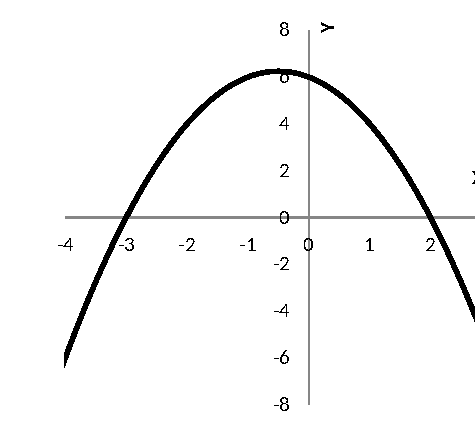
\includegraphics[width=2.15in,height=1.71in]{capitulos/funcao_do_segundo_grau/media/image30.pdf}
	\end{Center}
\end{figure}
\end{multicols}

\begin{multicols}{2}
d) Raízes: \textit{x\textsubscript{1}=-4; x\textsubscript{2}=2}. Intersecção com Y em (0,-8); Intersecção com X em (-4,0) e (2,0);      V=(-1,-9).

\begin{figure}[H]
	\begin{Center}
		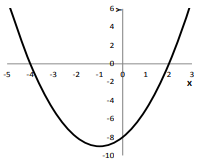
\includegraphics[width=2.15in,height=1.76in]{capitulos/funcao_do_segundo_grau/media/image31.png}
	\end{Center}
\end{figure}
\end{multicols}

\ansitem{}
\begin{multicols}{2}
a) Positiva $x<-1$ ou $x>1$; Negativa $-1 < x < 1$

\begin{figure}[H]
	\begin{Center}
		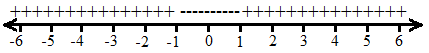
\includegraphics[width=2.65in,height=0.38in]{capitulos/funcao_do_segundo_grau/media/image32.png}
	\end{Center}
\end{figure}
\end{multicols}

\begin{multicols}{2}
b) Positiva \textit{x<-1} ou  \textit{x>3; }Negativa -1 <  \textit{x<3}

\begin{figure}[H]
	\begin{Center}
		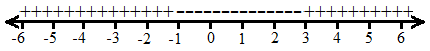
\includegraphics[width=2.66in,height=0.31in]{capitulos/funcao_do_segundo_grau/media/image33.png}
	\end{Center}
\end{figure}
\end{multicols}

\begin{multicols}{2}
c) Positiva \textit{-3} < \textit{x<2; }Negativa \textit{x<-3} ou \textit{x>2}

\begin{figure}[H]
	\begin{Center}
		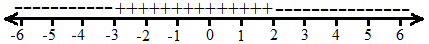
\includegraphics[width=2.62in,height=0.29in]{capitulos/funcao_do_segundo_grau/media/image34.png}
	\end{Center}
\end{figure}
\end{multicols}

\begin{multicols}{2}
d) Positiva \textit{x<-4} ou \textit{x>2}; Negativa \textit{-4 < } \textit{x <2}

\begin{figure}[H]
	\begin{Center}
		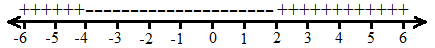
\includegraphics[width=2.57in,height=0.3in]{capitulos/funcao_do_segundo_grau/media/image35.png}
	\end{Center}
\end{figure}
\end{multicols}

\ansitem{}

\begin{figure}[H]
	\begin{Center}
		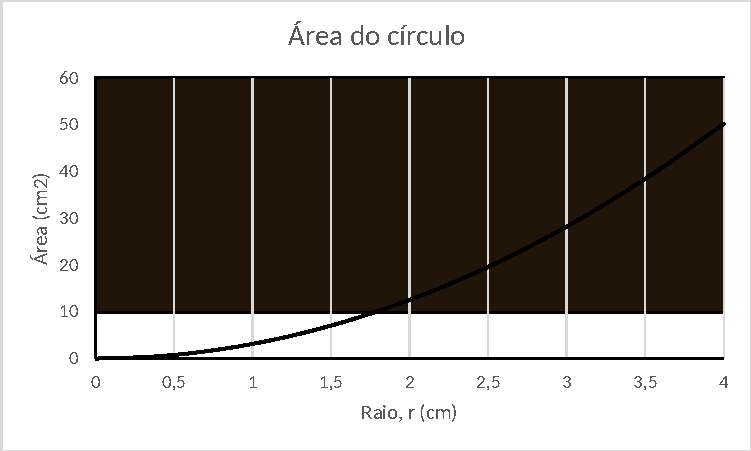
\includegraphics[width=2.71in,height=1.63in]{capitulos/funcao_do_segundo_grau/media/image36.pdf}
	\end{Center}
\end{figure}

\ansitem{} a) 1+10t-4.9t\textsuperscript{2} 

b) 

\begin{figure}[H]
	\begin{Center}
		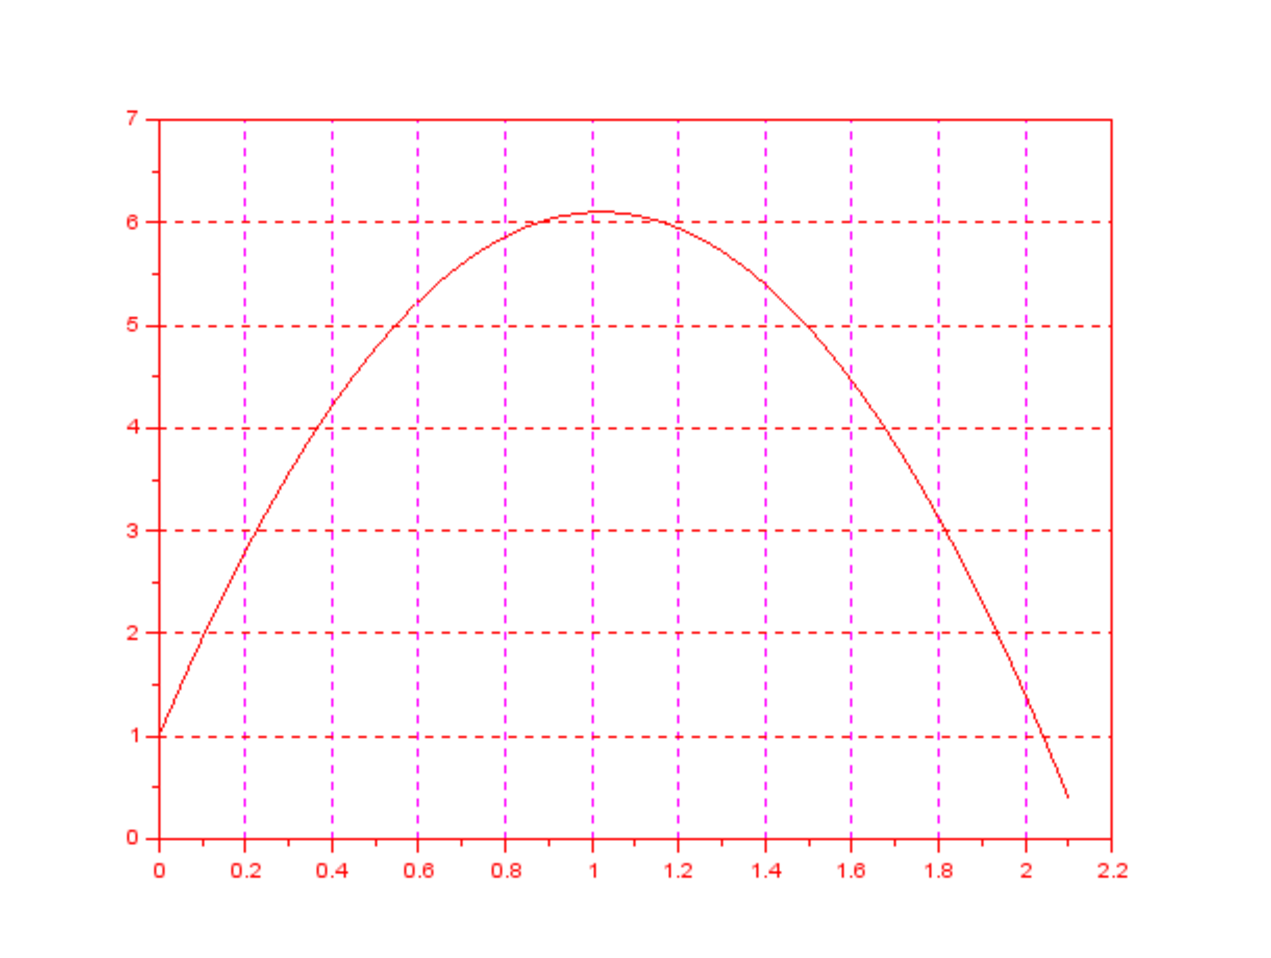
\includegraphics[width=2.71in,height=2.04in]{capitulos/funcao_do_segundo_grau/media/image37.pdf}
	\end{Center}
\end{figure}

	c) t=1,02 s

	d) ymáx = 6,102 m

	e) t = 2,13 s.

\ansitem{} a)  \( f \left( x \right) =x^{2}-5x+6 \)

    b) \( g \left( x \right) =x^{2}-7x+12 \) 

	c  \( h \left( x \right) =x^{2}+x-2 \)

	d)  \( i \left( x \right) =x^{2}+x-6 \)

\ansitem{} ~

\begin{multicols}{2}
\begin{figure}[H]
        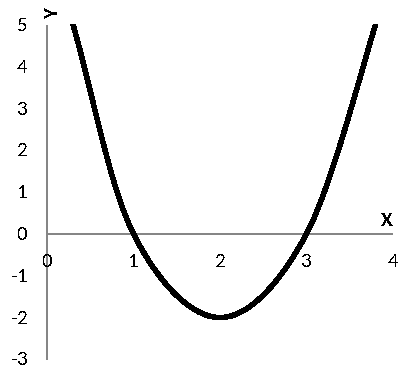
\includegraphics[width=2.19in,height=1.55in]{capitulos/funcao_do_segundo_grau/media/image38.pdf}
        
        (a)
\end{figure}

\begin{figure}[H]
        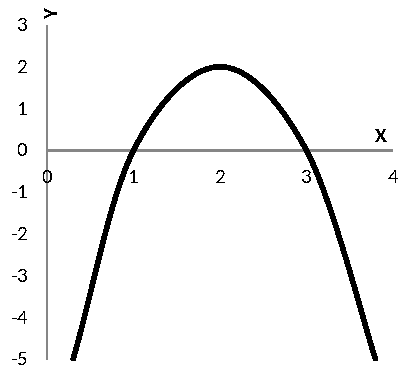
\includegraphics[width=2.2in,height=1.58in]{capitulos/funcao_do_segundo_grau/media/image39.pdf}
        
        (b)
\end{figure}

\begin{figure}[H]
        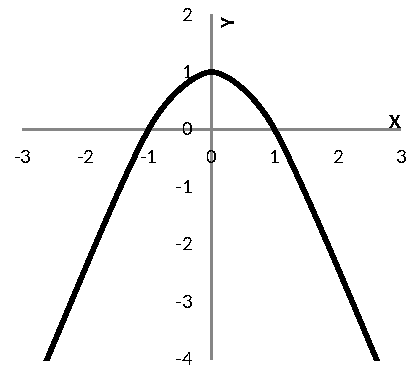
\includegraphics[width=2.2in,height=1.58in]{capitulos/funcao_do_segundo_grau/media/image40.pdf}
        
        (c)
\end{figure}

\begin{figure}[H]
        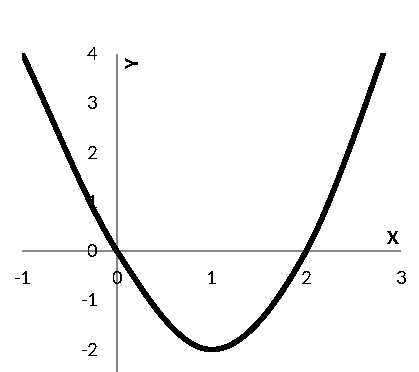
\includegraphics[width=2.2in,height=1.58in]{capitulos/funcao_do_segundo_grau/media/image41.pdf}
        
        (d)
\end{figure}
\end{multicols}

\ansitem{} a) \( f \left( x \right) =-x^{2}+2x \)

    b)  \( g \left( x \right) =x^{2}-4x+3 \) 

	b) \( h \left( x \right) = 2x^{2}-8x+6 \) 

	c) \( i \left( x \right) =-\frac{5}{4}x^{2}+5 \)

\ansitem{} ~

\begin{multicols}{2}
\begin{figure}[H]
        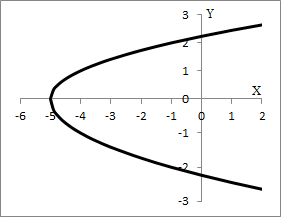
\includegraphics[width=2.05in,height=1.55in]{capitulos/funcao_do_segundo_grau/media/image42.png}
        
        (a)
\end{figure}

\begin{figure}[H]
        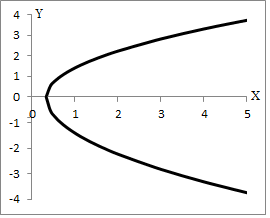
\includegraphics[width=2.06in,height=1.68in]{capitulos/funcao_do_segundo_grau/media/image43.png}
        
        (b)
\end{figure}

\begin{figure}[H]
        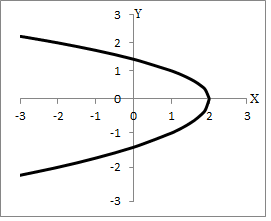
\includegraphics[width=1.99in,height=1.69in]{capitulos/funcao_do_segundo_grau/media/image44.png}
        
        (c)
\end{figure}

\begin{figure}[H]
        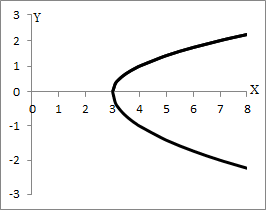
\includegraphics[width=2.03in,height=1.73in]{capitulos/funcao_do_segundo_grau/media/image45.png}
        
        (d)
\end{figure}

\begin{figure}[H]
        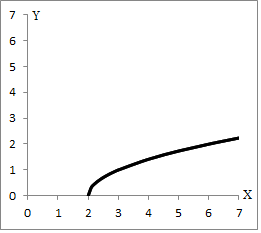
\includegraphics[width=1.99in,height=1.54in]{capitulos/funcao_do_segundo_grau/media/image46.png}
        
        (e)
\end{figure}

\begin{figure}[H]
        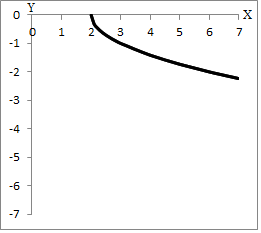
\includegraphics[width=1.99in,height=1.73in]{capitulos/funcao_do_segundo_grau/media/image47.png}
        
        (f)
\end{figure}

\begin{figure}[H]
        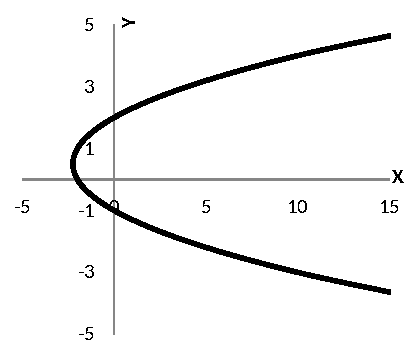
\includegraphics[width=1.99in,height=1.71in]{capitulos/funcao_do_segundo_grau/media/image48.pdf}
        
        (g)
\end{figure}

\begin{figure}[H]
        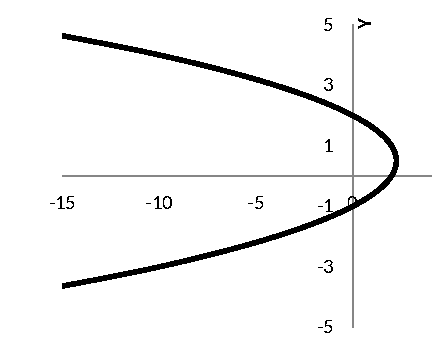
\includegraphics[width=1.96in,height=1.59in]{capitulos/funcao_do_segundo_grau/media/image49.pdf}
        
        (h)
\end{figure}
\end{multicols}

\ansitem{} a)  \( f \left( x \right) =-\frac{5}{2}x^{2}+5x \) 

\begin{table}[H]
    b)

    \centering
\begin{tabular}{p{0.27in}p{0.33in}}
\hline
%row no:1
\multicolumn{1}{|p{0.27in}}{x} & 
\multicolumn{1}{|p{0.33in}|}{y} \\
\hhline{--}
%row no:2
\multicolumn{1}{|p{0.27in}}{0} & 
\multicolumn{1}{|p{0.33in}|}{0} \\
\hhline{--}
%row no:3
\multicolumn{1}{|p{0.27in}}{1/2} & 
\multicolumn{1}{|p{0.33in}|}{1,875} \\
\hhline{--}
%row no:4
\multicolumn{1}{|p{0.27in}}{1} & 
\multicolumn{1}{|p{0.33in}|}{2,5} \\
\hhline{--}
%row no:5
\multicolumn{1}{|p{0.27in}}{3/2} & 
\multicolumn{1}{|p{0.33in}|}{1,875} \\
\hhline{--}
%row no:6
\multicolumn{1}{|p{0.27in}}{1} & 
\multicolumn{1}{|p{0.33in}|}{0} \\
\hhline{--}

\end{tabular}
 \end{table}

c)

\begin{figure}[H]
	\begin{Center}
		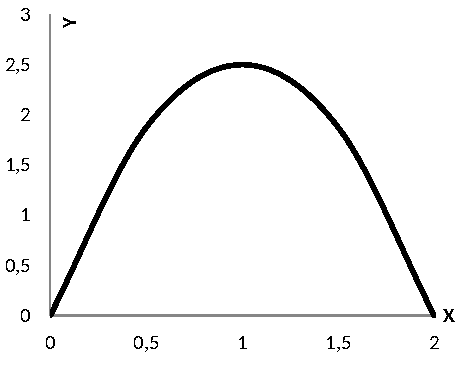
\includegraphics[width=2.45in,height=1.73in]{capitulos/funcao_do_segundo_grau/media/image50.pdf}
	\end{Center}
\end{figure}

\ansitem{} Lado do quadrado = 6,6159 m e raio do semicírculo = 3,3079 m.

\ansitem{} a) \textit{x = 1,22} e \textit{P\textsubscript{máx} = 3,107}.

b)

\begin{figure}[H]
	\begin{Center}
		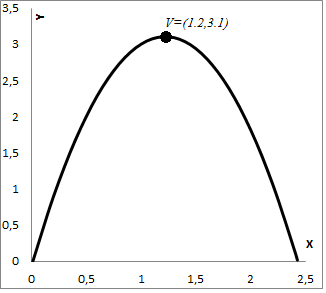
\includegraphics[width=2.52in,height=1.95in]{capitulos/funcao_do_segundo_grau/media/image51.png}
	\end{Center}
\end{figure}

\ansitem{} \( D=20 cm \).

\end{enumerate}